\paragraph{Example 1}{
\begin{lstlisting}[language=Python]
from BNumMet.Random import marsaglia_rand, clear_marsaglia_vars
clear_marsaglia_vars()
for i in range(10):
    print(marsaglia_rand(base=41, lag_r=2, lag_s=1, carry=0, seed_tuple=(0, 1)))

>>  0.975609756097561
    0.024390243902439025
    0.926829268292683
    0.0975609756097561
    0.8048780487804879
    0.2926829268292683
    0.4878048780487805
    0.8048780487804879
    0.6585365853658537
    0.12195121951219512
\end{lstlisting}
}
\paragraph{Example 2}{
\begin{lstlisting}[language=Python]
from BNumMet.Random import marsaglia_rand, clear_marsaglia_vars
clear_marsaglia_vars()
fail = [
    (
        marsaglia_rand(base=100, lag_r=2, lag_s=1, carry=0, seed_tuple=(0, 1)),
        marsaglia_rand(base=100, lag_r=2, lag_s=1, carry=0, seed_tuple=(0, 1)),
    )
    for i in range(100000)
]
plt.scatter(*zip(*fail), s=1, c="black")
\end{lstlisting}
\begin{figure}[H]
    \centering
    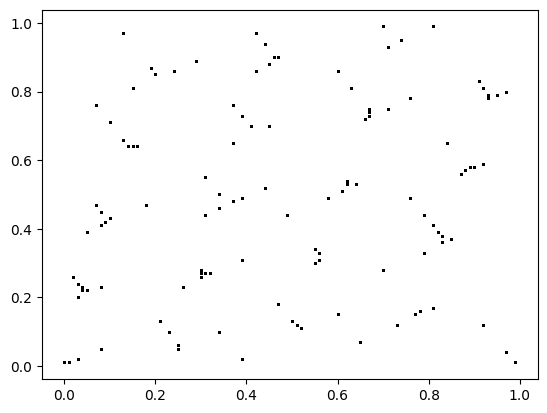
\includegraphics{Include/Images/Thesis/Documentation/Randomness/Marsaglia Rand Example 2.png}
    \caption{Marsaglia Rand Example 2}
    \label{fig:Marsaglia Rand Example 2}
\end{figure}
}
\paragraph{Example 3}{
\begin{lstlisting}[language=Python]
from BNumMet.Random import marsaglia_rand, clear_marsaglia_vars
clear_marsaglia_vars()
fail = [
    (
        marsaglia_rand(base=41, lag_r=2, lag_s=1, carry=0, seed_tuple=(0, 1)),
        marsaglia_rand(base=41, lag_r=2, lag_s=1, carry=0, seed_tuple=(0, 1)),
    )
    for i in range(100000)
]
plt.scatter(*zip(*fail), s=1, c="black")
\end{lstlisting}
\begin{figure}[H]
    \centering
    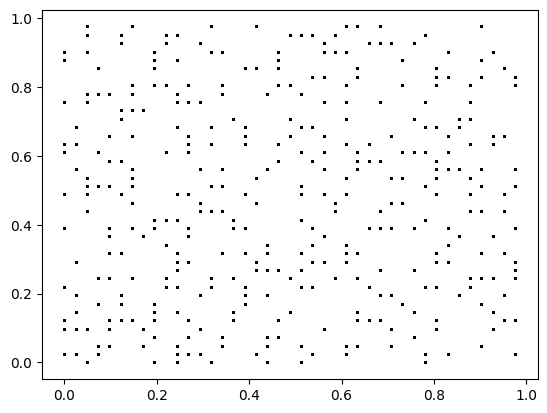
\includegraphics{Include/Images/Thesis/Documentation/Randomness/Marsaglia Rand Example 3.png}
    \caption{Marsaglia Rand Example 3}
    \label{fig:Marsaglia Rand Example 3}
\end{figure}
}
